O padrão \emph{Factory Method} está relacionado a todos os outros padrões que conduzam
algum tipo de construção encapsulada de objetos. Além de \emph{factory} os padrões Iterator,
Singleton , Builder, Prototype e Bridge- para citar alguns – estão relacionados ao padrão
\emph{Factory Method}.

Define uma interface para a criação de um objeto, mas deixa que as subclasses
decidam qual a classe instanciar. Permite a uma classe delegar a instanciação para as
subclasses.\cite{gamma95}


\subsection{Motivação}
\label{sub:fac_motiv}

\emph{Frameworks} usam classes abstratas para definir e manter relacionamentos entre
objetos. Um \emph{framework} é muitas vezes responsável por criar esses objetos também.

Considere-se um \emph{framework} de aplicações que podem apresentar vários documentos ao
usuário. Duas abstrações chave neste \emph{framework} são as classes Application e
Documento. Ambas as classes são abstratas, e os clientes têm usalas como subclasses para perceber
suas implementações de aplicações específicas. Para criar um aplicativo de desenho, por
exemplo, podemos definir as classes e \emph{DrawingApplication} e \emph{DrawingDocument}. A
classe Application é responsável pela gestão de documentos e como criá-los assim que o usuário selecione Open ou Novo a partir de um menu, por exemplo.\cite{gamma95}

Como subclasse do documento em particular para instanciar é específico do aplicativo,
a classe Application não consegue prever que documento deve criar, a classe Application só sabe quando um novo documento deve ser criado, não o tipo do documento para criar. Isso cria um dilema: O \emph{framework} deve instanciar classes, mas só sabe sobre classes abstratas, que não pode instanciar.\cite{gamma95}

O padrão \emph{Factory Method} oferece uma solução. Ele encapsula o conhecimento de
que subclasse Documento deve criar e move este conhecimento para fora do \emph{framework}.\cite{gamma95}

\begin{center}
	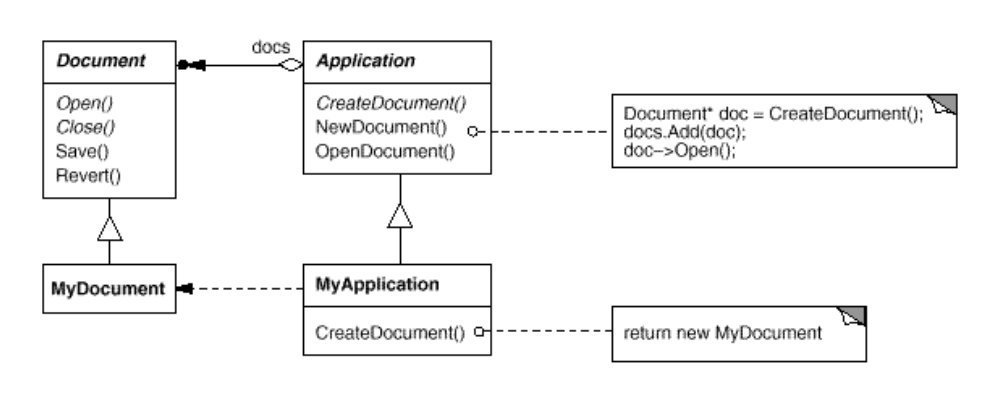
\includegraphics[scale=0.40]{Figuras/image1.jpg}
	\captionof{figure}{\label{diagrama1} Representação da estrutura para criação de documentos}
	\label{fig:diagrama1}
\end{center}

As subclasses da aplicação redefinem uma operação abstrata \emph{CreateDocument} no 
aplicativo para retornar a subclasse apropriada documento. Uma vez que uma subclasse da aplicação é instanciada, ele pode então instanciar documentos sem saber sua classe. Chamamos \emph{CreateDocument} um \emph{factory method} porque é
responsável por "produzir" um objeto.\cite{gamma95}

\subsection{Aplicação}
\label{sub:fac_aplica}

Se usa \emph{Factory pattern} quando:\cite{gamma95}

\begin{itemize}
	\item Quando uma classe (o criador) não pode antecipar a classe dos objetos que deve criar
.	\item uma classe quer que suas subclasses possam especificar os objetos que ele cria.
	\item Quando classes delegam responsabilidade para uma entre várias subclasses de apoio e
queremos localizar num ponto único a conhecimento de qual subclasse está sendo usada

\end{itemize}


\subsection{Problema}
\label{sub:fac_problema}

Uma classe precisa instanciar a derivação de uma outra, mas não sabe qual. O \emph{Factory Method} permite que uma classe derivada tome essa decisão.

\subsection{Solução}
\label{sub:fac_solucao}

Uma classe derivada decide qual classe instanciar e o modo como instanciá-la.
Algumas razões existem para que não queria utilizar new diretamente. A primeira, e
mais óbvia, é não saber que classe de objeto instanciar.
Isso é comum numa aplicação bem desenhada onde variáveis são estruturadas com
base em interfaces. Assim, vários tipos de objetos diferentes podem ser associados a
essa variável. Outra razão é a necessidade de inicializar o objeto instanciado antes de ser
atribuído à variável. Importante notar
que esta inicialização não depende do ambiente onde o objeto será utilizado, mas apenas
da estrutura do próprio objeto.\cite{fact1}\cite{gamma95}



\subsection{Como utilizar}
\label{sub:fac_utilizacao}

\begin{itemize}
	\item É possível criar um objeto sem ter conhecimento algum de sua classe concreta?
	\item Esse conhecimento deve estar em alguma parte do sistema, mas não precisa estar
no cliente
	\item \emph{FactoryMethod} define uma interface comum para criar objetos
	\item O objeto específico é determinado nas diferentes implementações dessa interface
	\item O cliente do \emph{FactoryMethod} precisa saber sobre implementações concretas do
objeto criador do produto desejado

\end{itemize}


\subsection{Diagrama de classes}
\label{sub:fac_diagrama}

\begin{center}
	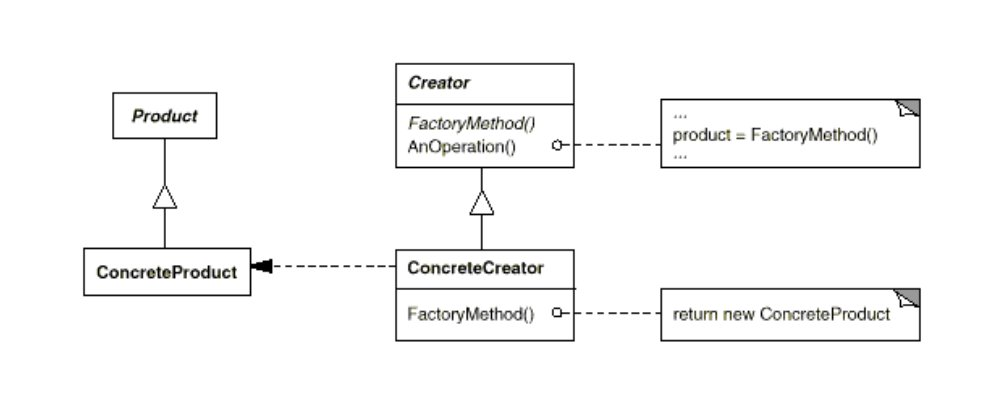
\includegraphics[scale=0.40]{Figuras/image2.jpg}
	\captionof{figure}{\label{diagrama2} Representação da estrutura de classes utilizando \emph{factory method}}
	\label{fig:diagrama2}
\end{center}

\begin{itemize}
	\item \emph{Product}: define a interface dos objetos criados pelo \emph{Factory Method}
	\item \emph{ConcreteProduct}: implementa a interface \emph{Product}
	\item \emph{Creator}: declara o \emph{Factory Method} que retorna um objeto do tipo \emph{Product}
		\begin{itemize}
			\item  Às vezes, o \emph{Creator} não é apenas uma interface, mas pode envolver uma
classe concreta que tenha uma implementação default para o \emph{Factory Method} para retornar um objeto com algum tipo \emph{ConcreteProduct} default
			\item Pode chamar o \emph{Factory Method} para criar um produto do tipo \emph{Product}
		\end{itemize}
	\item \emph{ConcreteCreator}: faz override do \emph{Factory Method} para retornar uma instância de \emph{ConcreteProduct}
\end{itemize}


\subsection{Exemplos de uso}
\label{sub:fac_uso}

\subsection{Benefícios}
\label{sub:fac_beneficios}

\begin{itemize}
	\item Criação de objetos é desacoplada do conhecimento do tipo concreto do objeto
	\item Conecta hierarquias de classe paralelas
	\item Facilita a extensibilidade
\end{itemize}

\emph{Factory Methods} eliminam a necessidade de colocar classes específicas da aplicação no código.\cite{fact2}

\begin{itemize}
	\item O código só lida com a interface \emph{Product}
	\item O código pode, portanto funcionar com qualquer classe \emph{ConcreteProduct} Provê ganchos (\emph{Hook Methods}) para subclasses.
	\item Criar objetos dentro de uma classe com um \emph{Factory Method} é sempre mais flexível do que criar objetos diretamente.
	\item O \emph{Factory Method} provê um gancho para que subclasses forneçam uma versão estendida de um objeto
\end{itemize}
